\documentclass[11pt,letterpaper]{article}
\setlength{\parindent}{0em}                  %DISTANCIA SANGRÍA
\setlength{\parskip}{0.5em}                  %DISTANCIA ENTRE PÁRRAFOS
\textwidth 6.5in
\textheight 9.in
\oddsidemargin 0in
\headheight 0in
\usepackage[T1]{fontenc}
\usepackage[dvipsnames]{xcolor}
\usepackage{fancybox}
\usepackage[utf8]{inputenc}
\usepackage{epsfig,graphicx}
\usepackage{multicol,pst-plot}
\usepackage{pstricks}
\usepackage{amsmath}
\usepackage{amsfonts}
\usepackage{amssymb}
\usepackage{eucal}
\usepackage[left=2cm,right=2cm,top=2cm,bottom=2cm]{geometry}
\usepackage{txfonts}
% \usepackage[spanish]{babel}
\usepackage[colorlinks]{hyperref}
\usepackage{cancel}
\usepackage{caption}
\usepackage{float}
\usepackage{upgreek}
\usepackage{gensymb}
\usepackage{subfigure}
\usepackage{siunitx}
\usepackage{color}
\usepackage{tikz}
\usepackage{listings}
\usepackage{minted}
\usepackage{mdframed}
\usepackage{natbib}
\usepackage{pifont}
\bibliographystyle{mnras}
\setcitestyle{aysep{","}}
\usepackage{multicol}
\renewcommand{\bibpreamble}{\begin{multicols}{2}}
\renewcommand{\bibpostamble}{\end{multicols}}
\renewcommand{\r}[1]{\textcolor{red}{#1}}
\setlength{\bibsep}{3pt}

%DEFINICIÓN DE COLORES EXTRAS

\definecolor{codegreen}{rgb}{0,0.6,0}
\definecolor{codegray}{rgb}{0.5,0.5,0.5}
\definecolor{backcolour}{rgb}{0.95,0.95,0.95}
\hypersetup{colorlinks=true,linkcolor=codegreen,citecolor=blue,filecolor=blue,urlcolor=magenta,}

%CONFIGURACIÓN DE LSTLISTINGS PARA CÓDIGOS

\lstset{ %
language=matlab,                % choose the language of the code
basicstyle=\footnotesize,       % the size of the fonts that are used for the code
numbers=left,                   % where to put the line-numbers
numberstyle=\footnotesize,      % the size of the fonts that are used for the line-numbers
stepnumber=1,                   % the step between two line-numbers. If it is 1 each line will be numbered
numbersep=5pt,                  % how far the line-numbers are from the code
backgroundcolor=\color{white},  % choose the background color. You must add \usepackage{color}
showspaces=false,               % show spaces adding particular underscores
showstringspaces=false,         % underline spaces within strings
showtabs=false,                 % show tabs within strings adding particular underscores
frame=single,                   % adds a frame around the code
tabsize=2,                      % sets default tabsize to 2 spaces
captionpos=b,                   % sets the caption-position to bottom
breaklines=true,                % sets automatic line breaking
breakatwhitespace=false,        % sets if automatic breaks should only happen at whitespace
escapeinside={\%*}{*)}          % if you want to add a comment within your code
}
\lstdefinestyle{mystyle}{
	backgroundcolor=\color{backcolour},   
	commentstyle=\color{red},
	keywordstyle=\bfseries\color{magenta},
	numberstyle=\tiny\color{codegray},
	stringstyle=\color{codegreen},
	basicstyle=\footnotesize\ttfamily,
	identifierstyle=\color{blue},
	breakatwhitespace=false,         
	breaklines=true,                 
	captionpos=b,                    
	keepspaces=true,                 
	numbers=left,                    
	numbersep=5pt,                  
	showspaces=false,                
	showstringspaces=false,
	showtabs=false,                  
	tabsize=2
}

\lstset{style=mystyle}

%CONFIGURACIÓN DE MINTED PARA CÓDIGOS

\usemintedstyle{vs}

%DEFINICIÓN DE COMANDOS EXTRAS

\pagestyle{empty}
\DeclareMathOperator{\tr}{Tr}                      %ICONO TRAZA MECANICA CUANTICA
\DeclareMathOperator{\rsol}{R_\odot}               %ICONO RADIO SOLAR
\DeclareMathOperator{\lsol}{L_\odot}               %ICONO LUMINOSIDAD SOLAR
\DeclareMathOperator{\msol}{M_\odot}               %ICONO MASA SOLAR
\DeclareMathOperator{\probabi}{Prob}               %ICONO PROBABILIDAD
\newcommand{\units}[1]{\left[ #1 \right]}          %CORCHETES PARA UNIDADES
\newcommand{\prob}[1]{\probabi\left( #1 \right)}   %OPERADOR PROBABILIDAD
\newcommand{\abs}[1]{\left|#1\right|}              %OPERADOR VALOR ABSOLUTO
\newcommand{\bra}[1]{\langle #1 |}                 %OPERADOR BRA
\newcommand{\ket}[1]{| #1 \rangle}                 %OPERADOR KET
\newcommand{\braket}[2]{\langle #1 | #2 \rangle}   %OPERADOR BRA-KET
\newcommand{\ketbra}[2]{|#1\rangle\langle#2|}      %OPERADOR KET-BRA
\newcommand{\mean}[1]{\langle #1 \rangle}          %PROMEDIO MECANICA CUANTICA
\newcommand{\eval}[3]{\left.#1\right|_{#2}^{#3}}   %COMANDO PARA EVALUAR INTEGRALES

%DEFINICIÓN DE REVISTAS CIENTÍFICAS

\newcommand\aap{A\&A}                % Astronomy and Astrophysics
\let\astap=\aap                          % alternative shortcut
\newcommand\aapr{A\&ARv}             % Astronomy and Astrophysics Review (the)
\newcommand\aaps{A\&AS}              % Astronomy and Astrophysics Supplement Series
\newcommand\actaa{Acta Astron.}      % Acta Astronomica
\newcommand\afz{Afz}                 % Astrofizika
\newcommand\aj{AJ}                   % Astronomical Journal (the)
\newcommand\ao{Appl. Opt.}           % Applied Optics
\let\applopt=\ao                         % alternative shortcut
\newcommand\aplett{Astrophys.~Lett.} % Astrophysics Letters
\newcommand\apj{ApJ}                 % Astrophysical Journal
\newcommand\apjl{ApJ}                % Astrophysical Journal, Letters
\let\apjlett=\apjl                       % alternative shortcut
\newcommand\apjs{ApJS}               % Astrophysical Journal, Supplement
\let\apjsupp=\apjs                       % alternative shortcut
% The following journal does not appear to exist! Disabled.
%\newcommand\apspr{Astrophys.~Space~Phys.~Res.} % Astrophysics Space Physics Research
\newcommand\apss{Ap\&SS}             % Astrophysics and Space Science
\newcommand\araa{ARA\&A}             % Annual Review of Astronomy and Astrophysics
\newcommand\arep{Astron. Rep.}       % Astronomy Reports
\newcommand\aspc{ASP Conf. Ser.}     % ASP Conference Series
\newcommand\azh{Azh}                 % Astronomicheskii Zhurnal
\newcommand\baas{BAAS}               % Bulletin of the American Astronomical Society
\newcommand\bac{Bull. Astron. Inst. Czechoslovakia} % Bulletin of the Astronomical Institutes of Czechoslovakia 
\newcommand\bain{Bull. Astron. Inst. Netherlands} % Bulletin Astronomical Institute of the Netherlands
\newcommand\caa{Chinese Astron. Astrophys.} % Chinese Astronomy and Astrophysics
\newcommand\cjaa{Chinese J.~Astron. Astrophys.} % Chinese Journal of Astronomy and Astrophysics
\newcommand\fcp{Fundamentals Cosmic Phys.}  % Fundamentals of Cosmic Physics
\newcommand\gca{Geochimica Cosmochimica Acta}   % Geochimica Cosmochimica Acta
\newcommand\grl{Geophys. Res. Lett.} % Geophysics Research Letters
\newcommand\iaucirc{IAU~Circ.}       % IAU Cirulars
\newcommand\icarus{Icarus}           % Icarus
\newcommand\japa{J.~Astrophys. Astron.} % Journal of Astrophysics and Astronomy
\newcommand\jcap{J.~Cosmology Astropart. Phys.} % Journal of Cosmology and Astroparticle Physics
\newcommand\jcp{J.~Chem.~Phys.}      % Journal of Chemical Physics
\newcommand\jgr{J.~Geophys.~Res.}    % Journal of Geophysics Research
\newcommand\jqsrt{J.~Quant. Spectrosc. Radiative Transfer} % Journal of Quantitiative Spectroscopy and Radiative Transfer
\newcommand\jrasc{J.~R.~Astron. Soc. Canada} % Journal of the RAS of Canada
\newcommand\memras{Mem.~RAS}         % Memoirs of the RAS
\newcommand\memsai{Mem. Soc. Astron. Italiana} % Memoire della Societa Astronomica Italiana
\newcommand\mnassa{MNASSA}           % Monthly Notes of the Astronomical Society of Southern Africa
\newcommand\mnras{MNRAS}             % Monthly Notices of the Royal Astronomical Society
\newcommand\na{New~Astron.}          % New Astronomy
\newcommand\nar{New~Astron.~Rev.}    % New Astronomy Review
\newcommand\nat{Nature}              % Nature
\newcommand\nphysa{Nuclear Phys.~A}  % Nuclear Physics A
\newcommand\pra{Phys. Rev.~A}        % Physical Review A: General Physics
\newcommand\prb{Phys. Rev.~B}        % Physical Review B: Solid State
\newcommand\prc{Phys. Rev.~C}        % Physical Review C
\newcommand\prd{Phys. Rev.~D}        % Physical Review D
\newcommand\pre{Phys. Rev.~E}        % Physical Review E
\newcommand\prl{Phys. Rev.~Lett.}    % Physical Review Letters
\newcommand\pasa{Publ. Astron. Soc. Australia}  % Publications of the Astronomical Society of Australia
\newcommand\pasp{PASP}               % Publications of the Astronomical Society of the Pacific
\newcommand\pasj{PASJ}               % Publications of the Astronomical Society of Japan
\newcommand\physrep{Phys.~Rep.}      % Physics Reports
\newcommand\physscr{Phys.~Scr.}      % Physica Scripta
\newcommand\planss{Planet. Space~Sci.} % Planetary Space Science
\newcommand\procspie{Proc.~SPIE}     % Proceedings of the Society of Photo-Optical Instrumentation Engineers
\newcommand\rmxaa{Rev. Mex. Astron. Astrofis.} % Revista Mexicana de Astronomia y Astrofisica
\newcommand\qjras{QJRAS}             % Quarterly Journal of the RAS
\newcommand\sci{Science}             % Science
\newcommand\skytel{Sky \& Telesc.}   % Sky and Telescope
\newcommand\solphys{Sol.~Phys.}      % Solar Physics
\newcommand\sovast{Soviet~Ast.}      % Soviet Astronomy (aka Astronomy Reports)
\newcommand\ssr{Space Sci. Rev.}     % Space Science Reviews
\newcommand\zap{Z.~Astrophys.}       % Zeitschrift fuer Astrophysik

%COMIENZA EL DOCUMENTO

\begin{document}

%CONFIGURACIÓN DEL ENCABEZADO

\usetikzlibrary{positioning}
\tikzset{every picture/.style={line width=0.75pt}}    
\pagestyle{plain}
\begin{flushleft}
Digital Image Processing\\
School of Information Science and Technology\\
\underline{ShanghaiTech University}
\end{flushleft}

% \begin{flushright}\vspace{-5mm}
% \includegraphics[height=1.5cm]{shanghaitech.jpg}
% \end{flushright}
 
\begin{center}\vspace{-1cm}
\textbf{\large Assignment 1}\\  
Due time: 23:59,	March 15th,	2023\\
\end{center}
\rule{\linewidth}{0.1mm}

\section{Notes}
This homework has \textbf{100 points} in total. \par
Please submit your homework to blackboard with a zip file named as \textcolor[rgb]{1,0,0}{\textbf{DIP2023\_ID\_Name\_hw1.zip}}. The zip file should contain three things: \textcolor[rgb]{1,0,0}{\textbf{a folder named 'codes' storing your codes}},  \textcolor[rgb]{1,0,0}{\textbf{a folder named 'images' storing the original images}}, and \textcolor[rgb]{1,0,0}{\textbf{your report named as report\_ID\_Name\_hw1.pdf}}. The names of your codes should look like \textcolor[rgb]{1,0,0}{\textbf{'p1a.m'}} (for (a) part of Problem $1$), so that we can easily match your answer to the question. \textcolor[rgb]{1,0,0}{Make sure all paths in your codes are relative path and we can get the result directly after running the code}. Please answer in \textcolor[rgb]{1,0,0}{English}. \par

Please complete all the coding assignments using \textcolor[rgb]{1,0,0}{MATLAB}. All core codes are required to be implemented \textcolor[rgb]{1,0,0}{by yourself} (without using relevant built-in functions). Make sure your results in the report are the same with the results of your codes. Please explain with notes at least at the key steps of your code.

\section{Policy on plagiarism}
This is an individual homework. You can discuss the ideas and algorithms, but you can neither read, modify, and submit the codes of other students, nor allow other students to read, modify, and submit your codes. Do not directly copy ready-made or automatically generated codes, or your score will be seriously affected. We will check plagiarism using automated tools and any violations will result in a zero score for this assignment. 

\clearpage

\section{Problem sets}

\subsection*{Problem 1 (30 pts)}
$$
\begin{bmatrix}
6 & 1 & 2 & 1 & (2)\\ 
2 & 3 & 5 & 3 & 8\\ 
1 & 0 & 1 & 2 & 3\\ 
3 & 2 & 4 & 5 & 2\\ 
(1) & 5 & 3 & 4 & 0
\end{bmatrix}
$$
\begin{itemize}
\item[(a)] Calculate the $D_4,D_8,D_m$ distance between the pair of points(framed in parentheses) in the matrix above, mark the shortest 4-,8-,m-path respectively. Show the results in your report. (V=1,2,3) (10 pts)

\item[(b)] An affine transformation of coordinates is given by
$$
\begin{bmatrix}
x'
\\ 
y'
\\ 
1
\end{bmatrix}
=A\begin{bmatrix}
x\\ y\\ 1
\end{bmatrix}
=\begin{bmatrix}
a_{11} & a_{12} & a_{13}\\ 
a_{21} & a_{22} & a_{23}\\ 
0 & 0 & 1
\end{bmatrix}\begin{bmatrix}
x\\y 
\\ 1
\end{bmatrix}
$$
Please perform the following transformation on \textbf{jetplane.tif}, write out the affine transformation matrix, then show the results:

(1) Scaling and shearing. Set x-scaling factor to 2 and y-scaling factor to 3, then shear the image horizontally 4
units. (5 pts)

(2) Translation and Rotation. Move 2 units to the left and move down 5 units, then rotate 45 degrees clockwise
(about the origin). (5 pts)

(\textcolor[rgb]{1,0,0}{Hint:} The main focus of this problem is to solve the affine transformation matrix, and using built-in functions like imwarp() to obtain the transformed image is allowed.)
\item[(c)] Perform bit-plane slicing on \textbf{lena\_gray\_256.tif} to get bit plane 1-8 and show the results in your report. Which kind of bit-plane usually contains more effective information, low bit or high bit? Why? (10 pts)
\end{itemize}

\textbf{Solution:}
\begin{itemize}
	\item [(a)]\par {\bf 4-path:} The path is shown in the following matrix with red marks:
	\[\begin{bmatrix}
		6 & \r{1} & \r{2} & \r{1} & \r{2}\\ 
		\r{2} & \r{3} & 5 & 3 & 8\\ 
		\r{1} & 0 & 1 & 2 & 3\\ 
		\r{3} & 2 & 4 & 5 & 2\\ 
		\r{1} & 5 & 3 & 4 & 0
		\end{bmatrix}\] So the $D_4$ distance is 8.
	
	\par {\bf 8-path:} The path is shown in the following matrix with red marks:
	\[\begin{bmatrix}
		6 & 1 & 2 & 1 & \r{1}\\ 
		2 & 3 & 5 & \r{3} & 8\\ 
		1 & 0 & \r{1} & 2 & 3\\ 
		3 & \r{2} & 4 & 5 & 2\\ 
		\r{1} & 5 & 3 & 4 & 0
		\end{bmatrix}\] So the $D_8$ distance is 4.
	
	\par {\bf m-path:} The path is shown in the following matrix with red marks:
	\[\begin{bmatrix}
		6 & \r{1} & \r{2} & \r{1} & \r{1}\\ 
		\r{2} & \r{3} & 5 & 3 & 8\\ 
		\r{1} & 0 & 1 & 2 & 3\\ 
		\r{3} & 2 & 4 & 5 & 2\\ 
		\r{1} & 5 & 3 & 4 & 0
		\end{bmatrix}\] So the $D_m$ distance is 8.
	\item [(b)]
	\begin{itemize}
		\item [(1)] The coordinate of point $(x,y)$ after scaling with x-scaling factor 2 and y-scaling factor 3 is $(2x, 3y)$, then the scaling matrix is
		$\begin{bmatrix}
			2 & 0 & 0\\
			0 & 3 & 0\\
			0 & 0 & 1
		\end{bmatrix}$. Moreover, the coordinate of point $(x,y)$ after shearing in y-axis direction with 4 units is $(x, 4x + y)$, then the shearing matrix is
		$\begin{bmatrix}
			1 & 0 & 0\\
			4 & 1 & 0\\
			0 & 0 & 1
		\end{bmatrix}$.
		Therefore, the whole affine transform matrix is 
		$\begin{bmatrix}
			1 & 0 & 0\\
			4 & 1 & 0\\
			0 & 0 & 1
		\end{bmatrix}
		\times 
		\begin{bmatrix}
		2 & 0 & 0\\
		0 & 3 & 0\\
		0 & 0 & 1
		\end{bmatrix}
		=
		\begin{bmatrix}
			2 & 0 & 0\\
			8 & 3 & 0\\
			0 & 0 & 1
		\end{bmatrix}$.
		\par The processed result is shown in Figure~\ref{fig:SS}.
		\begin{figure}[b]
			\centering
			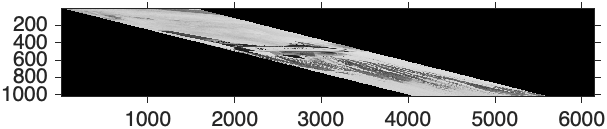
\includegraphics[width=0.7\textwidth]{images/p1b/SS.png}
			\caption{Image after scaling and shearing}
			\label{fig:SS}
			\centering
			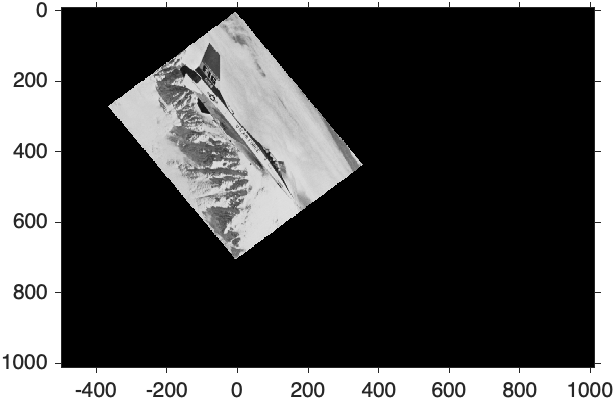
\includegraphics[width=0.5\textwidth]{images/p1b/TR.png}
			\caption{Image after translation and rotation}
			\label{fig:TR}
			\centering
			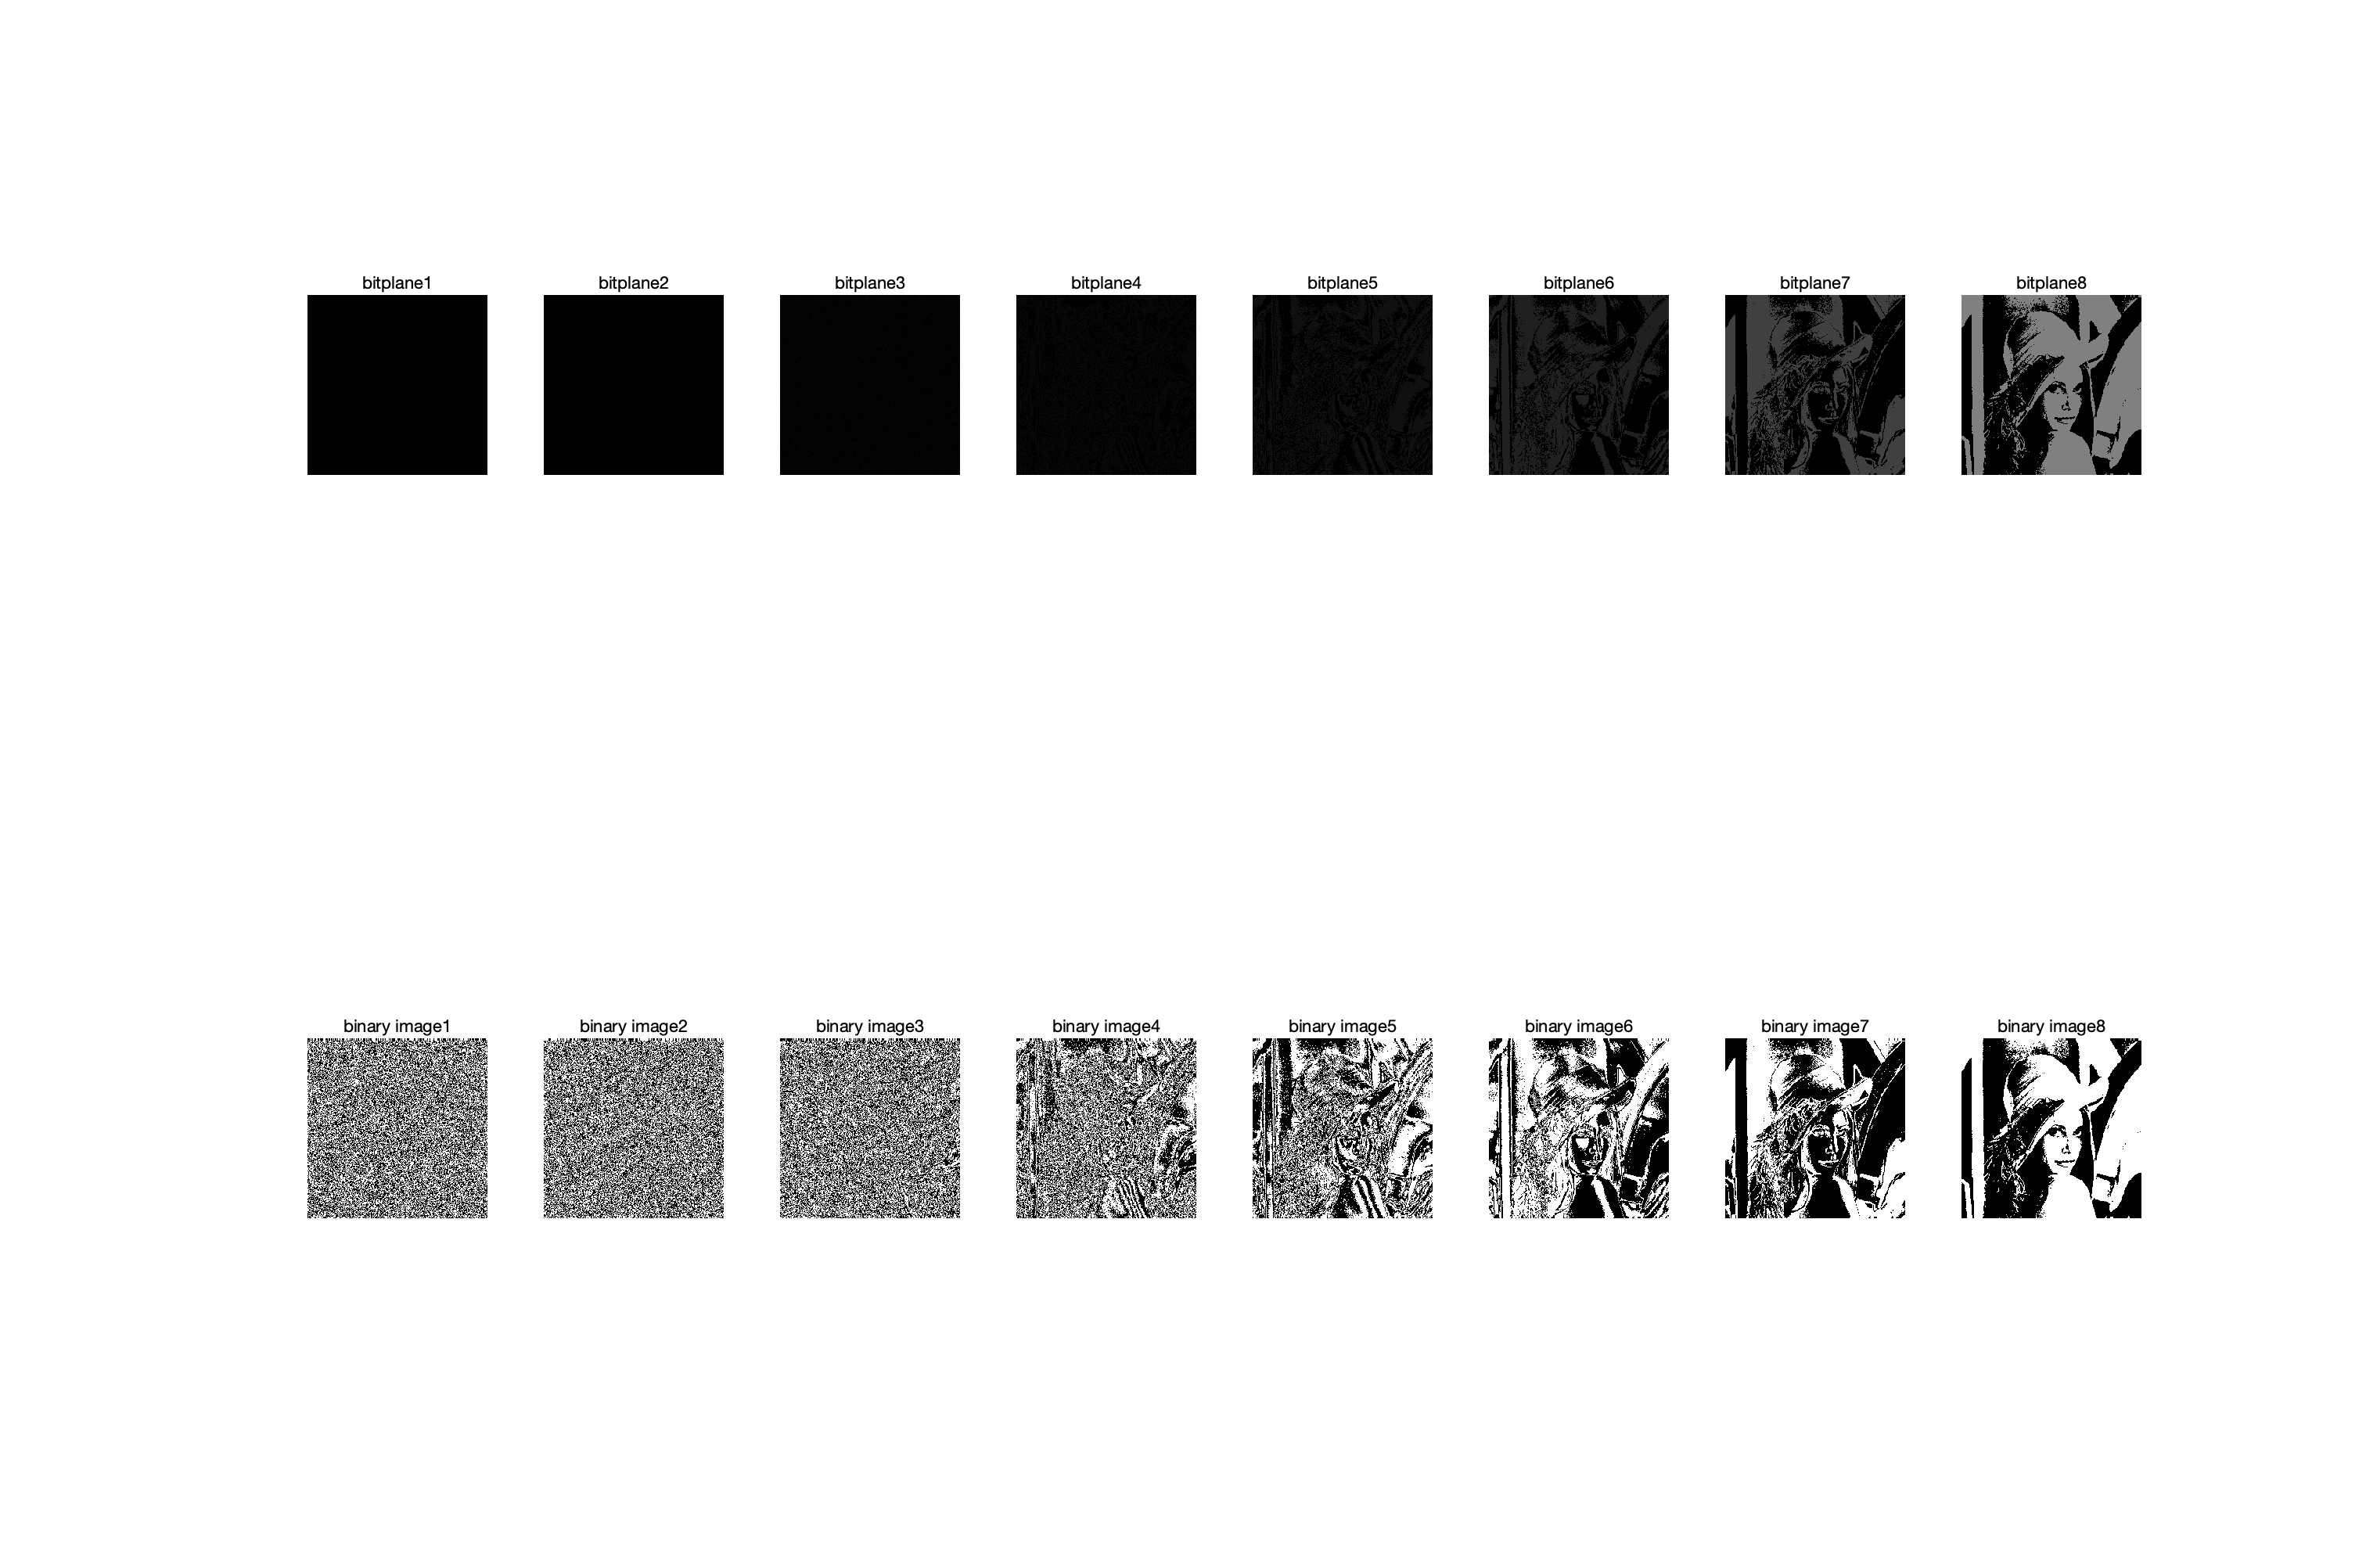
\includegraphics[width=1\textwidth]{images/p1c/bitplanes.png}
			\caption{Bitplanes slicing results. The top line shows the bitplanes with original values $0$ or $2^i$ and the bottom line shows the binary map with rescaled values $0$ or $255$.}
			\label{fig:bitplane}
		\end{figure}
		\item [(2)] The coordinate of point $(x,y)$ after translation is $(x+5, y-2)$, so the translation matrix is 
		$\begin{bmatrix}
			1 & 0 & 5\\
			0 & 1 & -2\\
			0 & 0 & 1
		\end{bmatrix}$. As for rotation, the coordinate of point $(x,y)$ after rotation $45\degree$ clockwise is $(x\cos 45\degree + y\sin 45\degree, y\cos 45\degree - x\sin 45\degree)$, so
		the rotation matrix is 
		$\begin{bmatrix}
			\cos 45\degree & \sin 45\degree & 0\\
			-\sin 45\degree & \cos 45\degree & 0\\
			0 & 0 & 1 
		\end{bmatrix}$
		Therefore, the whole affine transform matrix is 
		$\begin{bmatrix}
			1 & 0 & 5\\
			0 & 1 & -2\\
			0 & 0 & 1			
		\end{bmatrix}
		\times
		\begin{bmatrix}
			\frac{\sqrt{2}}{2} & \frac{\sqrt{2}}{2} & 0\\
			-\frac{\sqrt{2}}{2} & \frac{\sqrt{2}}{2} & 0\\
			0 & 0 & 1 
		\end{bmatrix}
		=
		\begin{bmatrix}
			\frac{\sqrt{2}}{2} & \frac{\sqrt{2}}{2} & 5\\
			-\frac{\sqrt{2}}{2} & \frac{\sqrt{2}}{2} & -2\\
			0 & 0 & 1	
		\end{bmatrix}$.
		The processed result is shown in Figure~\ref{fig:TR}.
		\item [(c)] The result is shown in Figure~\ref{fig:bitplane}.
		From the result, it is obvious that the high bits have more effective information since those high bits slices contain more semantic and structural information while those low bits slices contain almost noise.
	\end{itemize}
\end{itemize}


\clearpage

\subsection*{Problem 2 (30 pts)}
\begin{itemize}
\item[(a)] Compute the histogram of \textbf{einstein\_low\_contrast.tif}. Perform histogram equalization (HE) on it, show the result. Show the histogram of the processed image, too. Why can HE enhance the contrast? (10 pts)

\item[(b)] Match the histgram of \textbf{lena\_color.tif} to \textbf{peppers\_color.tif}. Show the result in your report. (8 pts)

\item[(c)] Perform contrast limited adptive histogram equalization(CLAHE) on \textbf{man\_in\_house.png}. Contrast the result to HE method. Show the results in your report. Explain why CLAHE has a better effect.(Reference: http://cas.xav.free.fr/Graphics\%20Gems\%204\%20-\%20Paul\%20S.\%20Heckbert.pdf, 
 page474-485) (12 pts)

(\textcolor[rgb]{1,0,0}{Hint:} If you can effectively eliminate the checkerboard effect and balance the efficiency of the algorithm, you will get a bonus. Built-in functions like hist(), histogram(), histeq() and adapthisteq() are not allowed.)
\end{itemize}

\textbf{Solution:}
\begin{itemize}
	\item [(a)] The histogram of input image is shown in Figure~\ref{fig:img_hist}, the result after HE is shown in Figure~\ref{fig:HE_res} and the histogram of result is shown in Figure~\ref{fig:res_hist}. 
		\par The reason why HE can enhance the contrast is that HE transforms the original image distribution into a nearly uniform distribution, which enlarges the intensity difference of area where its original contrast is low.
	\begin{figure}
		\centering
		\subfigure[Histogram of input imag]{
			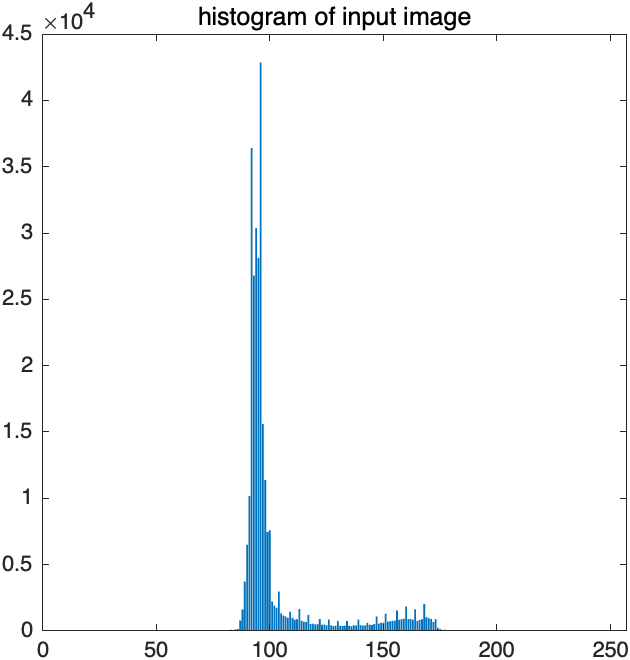
\includegraphics[width=0.4\textwidth]{images/p2a/img_hist.png}
			\label{fig:img_hist}
		}
		\subfigure[Histogram of result image]{
			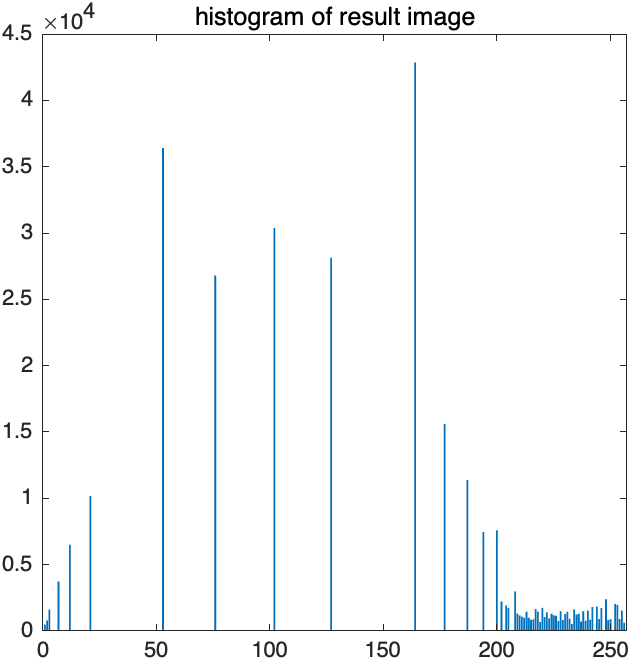
\includegraphics[width=0.4\textwidth]{images/p2a/res_hist.png}
			\label{fig:res_hist}
		}
		\subfigure[Result after HE]{
			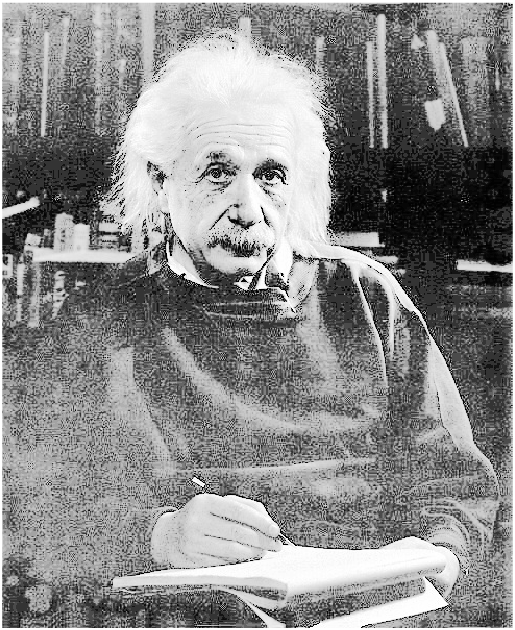
\includegraphics[width=0.5\textwidth]{images/p2a/HE_res.png}
			\label{fig:HE_res}
		}
		\caption{}
	\end{figure}
	\item [(b)] The result after histogram matching is shown in Figure~\ref{fig:hist_match}.

	\begin{figure}
		\centering
		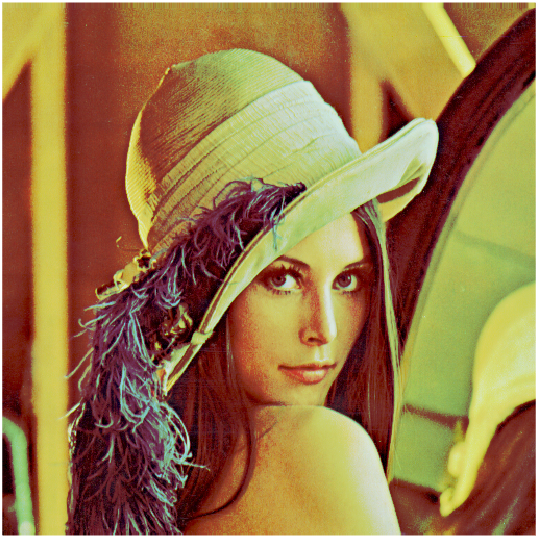
\includegraphics[width=0.5\textwidth]{images/p2b/hist_match.png}
		\caption{Histogram matching result}
		\label{fig:hist_match}
	\end{figure}

	\item [(c)] The result of HE and CLAHE are shown in Figure~\ref{fig:man_in_house_HE_res} and~\ref{fig:CLAHE_res}. 
	The detailed parameter settings of CLAHE are as follows:
	\begin{itemize}
		\item padding (mirroring) size = 30 pixels
		\item updated patch length = 2 pixels
		\item clipping limit = 0.3 (for distribution, not histogram)
	\end{itemize}
	The reasons why CLAHE has a better effect lie in two aspects:
	\begin{itemize}
		\item CLAHE only cares about the intensity distribution under the moving window, those local 
		distributions prevent pixels to be updated from being affected by other dense-intensity areas which are far away from them,
		so the areas where the contrast is low can get higher contrast.
		\item CLAHE limits the slop of histogram, this property prohibits too dense distribution after HE, which reduces artifacts like shining. 
	\end{itemize}
	\begin{figure}
		\centering
		\subfigure[HE result]{
			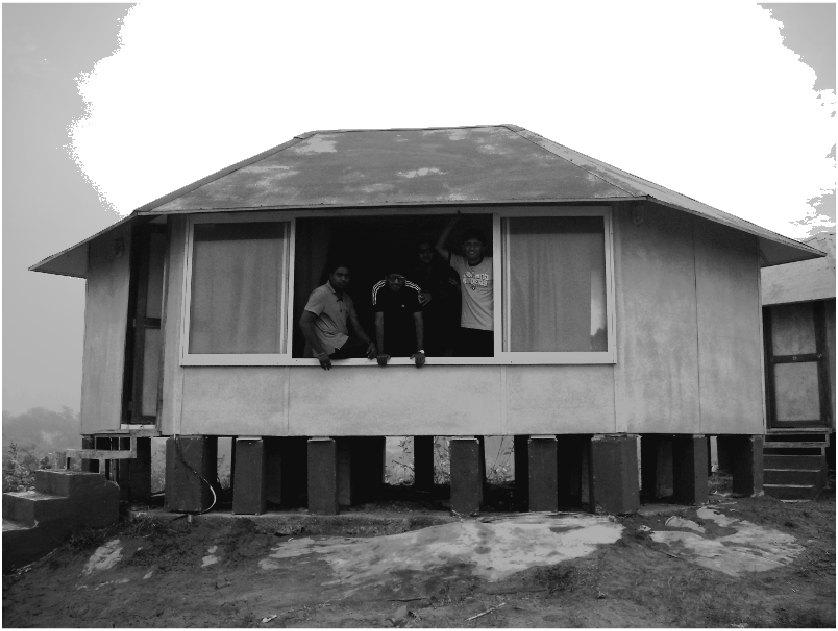
\includegraphics[width=0.45\textwidth]{images/p2c/HE_res.png}
			\label{fig:man_in_house_HE_res}
		}
		\subfigure[CLAHE result]{
			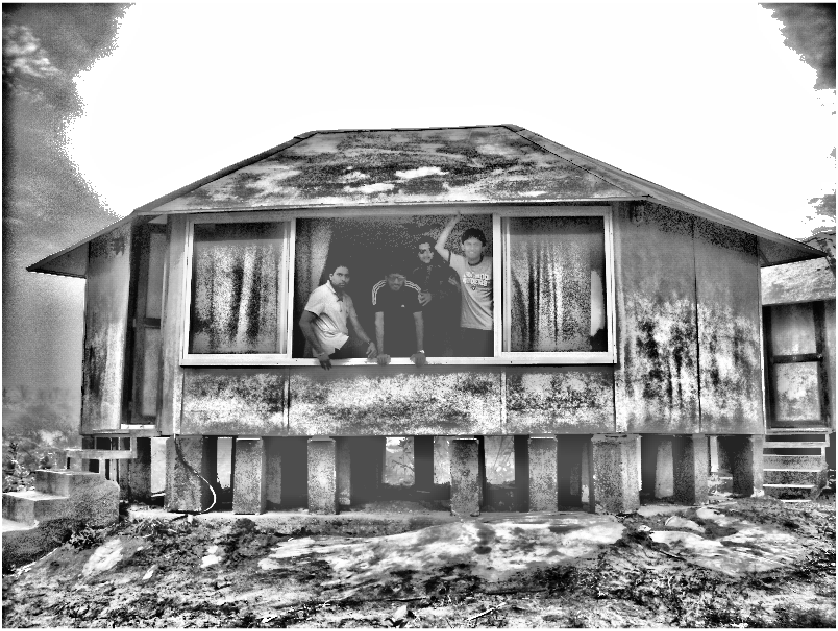
\includegraphics[width=0.45\textwidth]{images/p2c/CLAHE_res.png}
			\label{fig:CLAHE_res}
		}
		\caption{}
	\end{figure}
\end{itemize}
\clearpage

\subsection*{Problem 3 (40 pts)}

\begin{itemize}
    \item[(a)] Implement full convolution and cropped convolution of the given matrices, show the results in your report. (8 pts)
    
$$
 \begin{bmatrix}
6 & 4 & -1 & 0 & 1\\ 
1 & -3 & -4 & 3 & 2\\ 
0 & 3 & 5 & -2 & 1\\ 
9 & -1 & -3 & 4 & 5\\ 
-2 & -5 & 2 & 3 & 0
\end{bmatrix}\quad
\begin{bmatrix}
1 & 2 & 4\\ 
-3 & -1 & 1\\ 
5 & 2 & -1
\end{bmatrix}
$$

(\textcolor[rgb]{1,0,0}{Hint:} Pay attention to the difference between convolution and correlation.)

    \item[(b)] Describe the noise type on \textbf{circuitboard-a.tif}, \textbf{circuitboard-b.tif}, \textbf{circuitboard-c.tif} and \textbf{circuitboard-d.tif}, then choose the best filter you think for each of them to reduce the noise. Show the results in your report. (12 pts)

    (\textcolor[rgb]{1,0,0}{Hint:} Choose the best kernel size you think.)

    \item[(c)] Filter the image \textbf{house.tif} in both x direction and y direction with 3*3 Sobel mask and Laplacian mask. Show the results in your report. (8 pts)

    \item[(d)] Perform image sharpening on \textbf{house.tif} using LoG filter(with the $\sigma^2 = 1$ and another two values you choose yourself) and unsharpen mask method(choose the best $k$ you think). Show the results in your report. (12 pts)
\end{itemize}

\textbf{Solution:}
\begin{itemize}
	\item [(a)] The full convolution result is 
	\[\begin{bmatrix}
		6 	& 	16 	& 	31 	& 	14 	& 	-3 	& 	2 	& 	4 \\
		-17 & 	-19 & 	-1	& 	-12	& 	-12 & 	15 	& 	9 \\
		27 	& 	43 	& 	24	& 	6	& 	10 	& 	-3 	& 	5 \\
		14	& 	-5 	& 	-14	& 	8	& 	25 	& 	24 	& 	19\\
		-29	& 	10 	& 	54	& 	14	& 	-12	& 	15 	& 	4 \\
		51	& 	0 	& 	-39	& 	9	& 	35	&	9	& 	-5\\
		-10	& 	21 	& 	22	& 	14	& 	4	& 	-3	& 	0 \\
	\end{bmatrix}\]
	and the cropped convolution result is 
	\[\begin{bmatrix}
		-19 & 	-1	& 	-12	& 	-12 & 	15 	\\
		43 	& 	24	& 	6	& 	10 	& 	-3 	\\
		-5 	& 	-14	& 	8	& 	25 	& 	24 	\\
		10 	& 	54	& 	14	& 	-12	& 	15 	\\
		0 	& 	-39	& 	9	& 	35	&	9	\\
	\end{bmatrix}\]
	The detailed implementation is shown in the file: codes/p3a.mlx.
	\item [(b)] 
	\begin{itemize}
		\item circuitboard-a.tif: Peper noise (histogram shown in~\ref{fig:hist_a}) $\to$ max filter, result shown in~\ref{fig:res_a}.
		\item circuitboard-b.tif: Salt noise (histogram shown in~\ref{fig:hist_b}) $\to$ min filter, result shown in~\ref{fig:res_b}.
		\item circuitboard-c.tif: Salt-and-pepper noise (histogram shown in~\ref{fig:hist_c})$\to$ median filter, result shown in~\ref{fig:res_c}.
		\item circuitboard-d.tif: Gaussian noise (histogram shown in~\ref{fig:hist_d})$\to$ smooth filter, result shown in~\ref{fig:res_d}.
	\end{itemize}
	{\bf Remark:} All the kernels have size $3\times 3$.
	\begin{figure}
		\centering
		\subfigure[Histogram of circuitboard-a.tif]{
			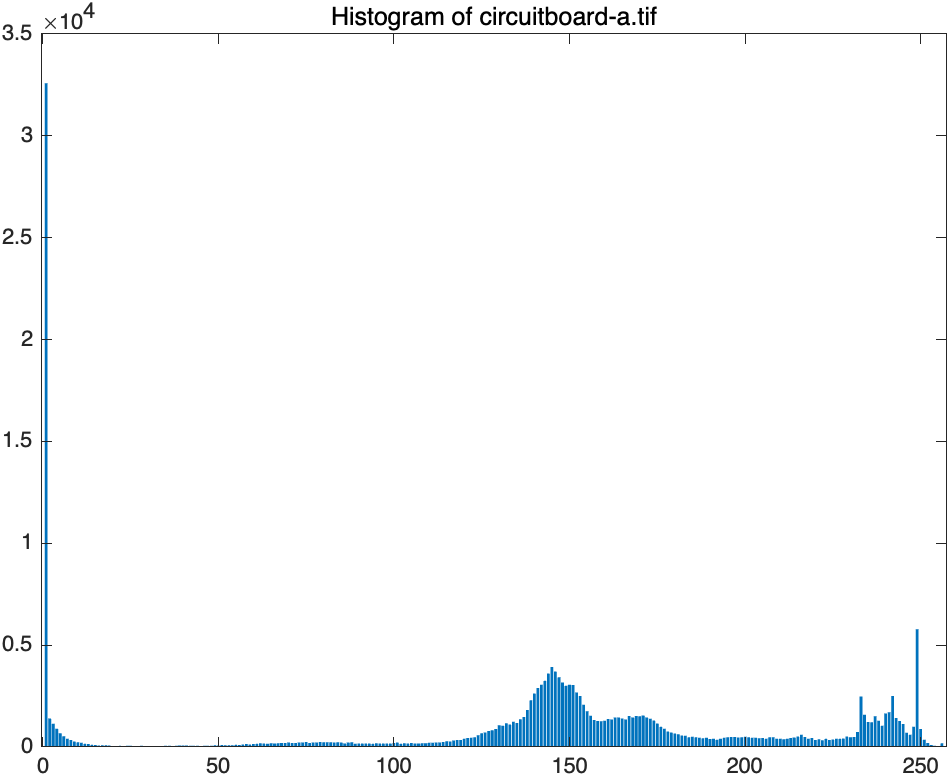
\includegraphics[width=0.4\textwidth]{images/p3b/hist_a.png}
			\label{fig:hist_a}
		}
		\subfigure[Histogram of circuitboard-b.tif]{
			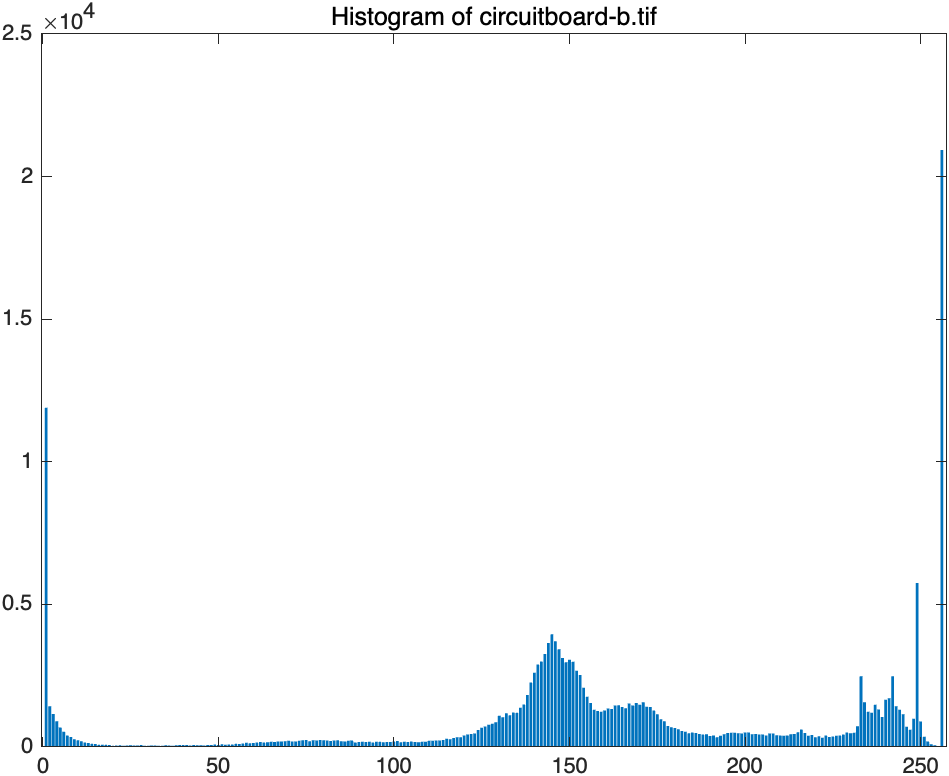
\includegraphics[width=0.4\textwidth]{images/p3b/hist_b.png}
			\label{fig:hist_b}
		}		
		\subfigure[Histogram of circuitboard-c.tif]{
			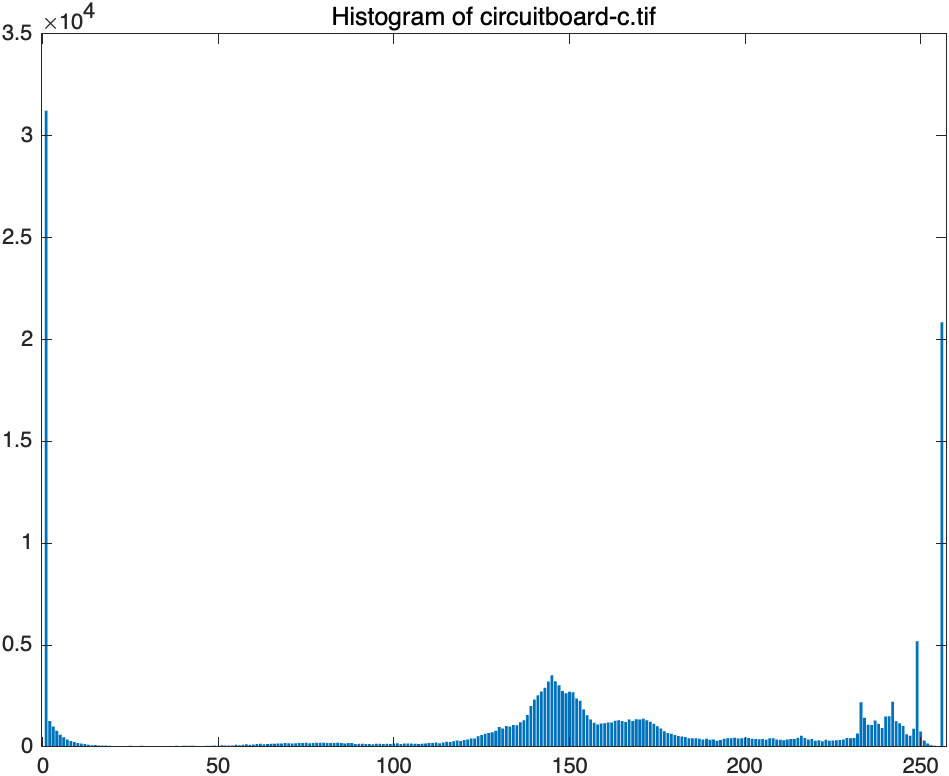
\includegraphics[width=0.4\textwidth]{images/p3b/hist_c.png}
			\label{fig:hist_c}
		}		
		\subfigure[Histogram of circuitboard-d.tif]{
			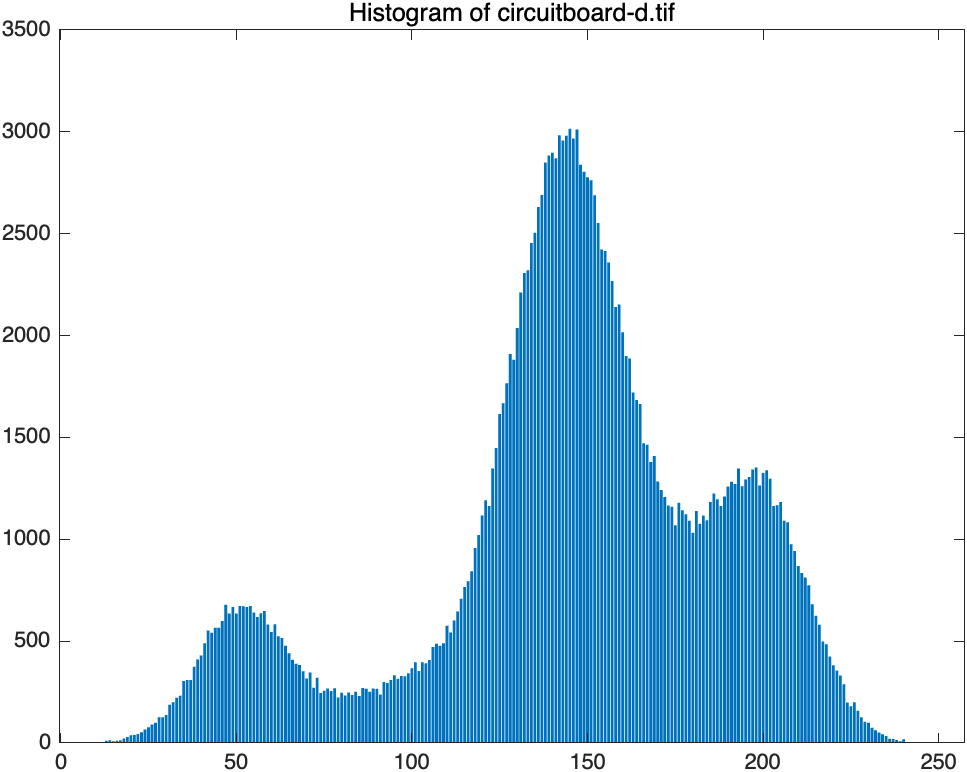
\includegraphics[width=0.4\textwidth]{images/p3b/hist_d.png}
			\label{fig:hist_d}
		}
		\caption{}
	\end{figure}
	\begin{figure}
		\centering
		\subfigure[denoised result after max filter]{
			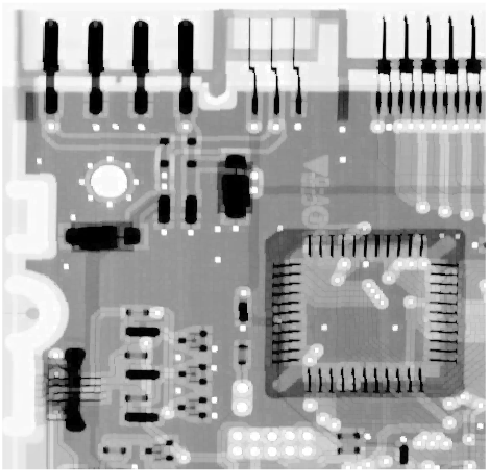
\includegraphics[width=0.4\textwidth]{images/p3b/res_a.png}
			\label{fig:res_a}
		}
		\subfigure[denoised result after min filter]{
			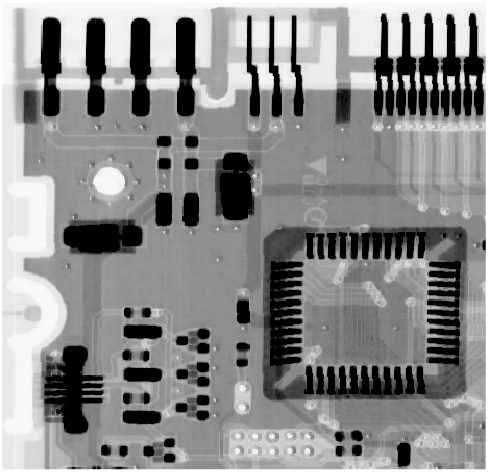
\includegraphics[width=0.4\textwidth]{images/p3b/res_b.png}
			\label{fig:res_b}
		}
		\subfigure[denoised result after median filter]{
			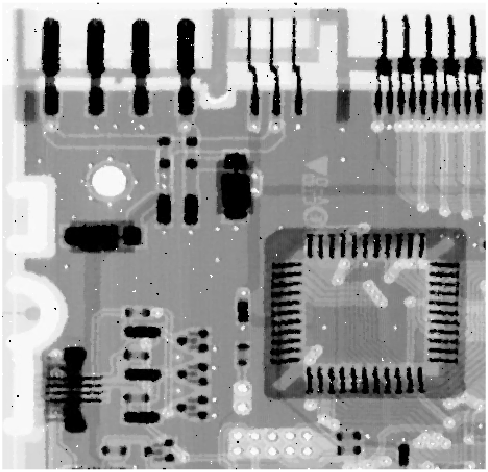
\includegraphics[width=0.4\textwidth]{images/p3b/res_c.png}
			\label{fig:res_c}
		}
		\subfigure[denoised result after smooth filter]{
			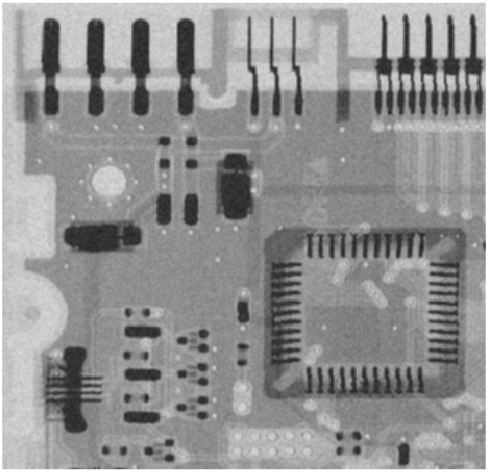
\includegraphics[width=0.4\textwidth]{images/p3b/res_d.png}
			\label{fig:res_d}
		}
		\caption{}
	\end{figure}
	\item [(c)] Results after applying Sobel mask and Laplacian mask are shown in~\ref{fig:sobel_res_x},~\ref{fig:sobel_res_y},~\ref{fig:laplacian_res_x} and~\ref{fig:laplacian_res_y} respectively.
	\begin{figure}
		\centering
		\subfigure[Result after applying Sobel mask in x direction]{
			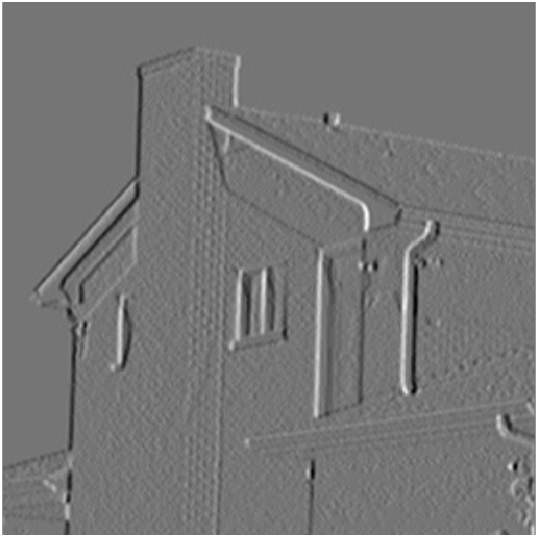
\includegraphics[width=0.4\textwidth]{images/p3c/sobel_res_x.png}
			\label{fig:sobel_res_x}
		}
		\subfigure[Result after applying Sobel mask in y direction]{
			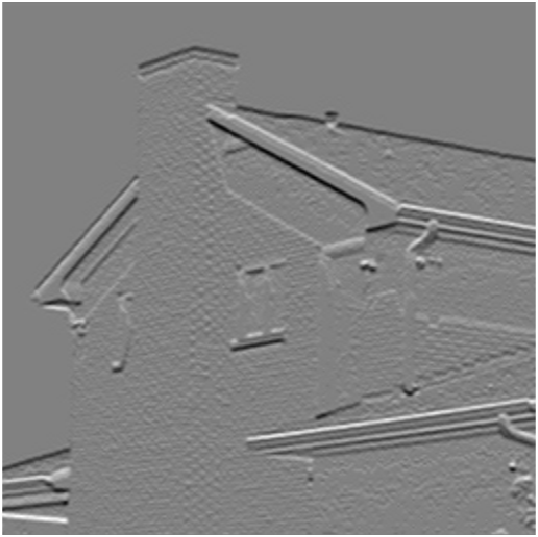
\includegraphics[width=0.4\textwidth]{images/p3c/sobel_res_y.png}
			\label{fig:sobel_res_y}
		}
		\subfigure[Result after applying Laplacian mask in x direction]{
			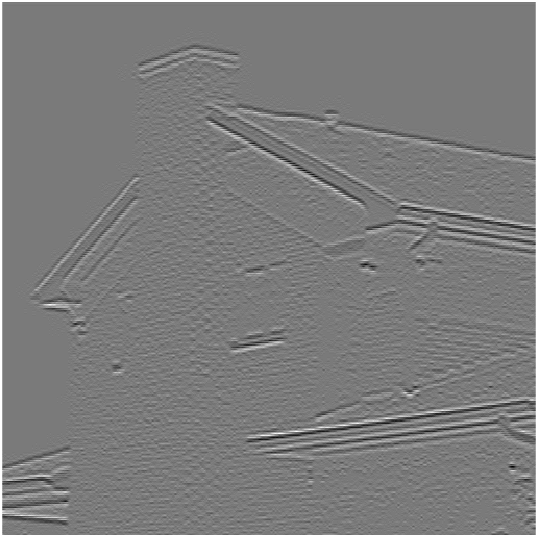
\includegraphics[width=0.4\textwidth]{images/p3c/laplacian_res_x.png}
			\label{fig:laplacian_res_x}
		}
		\subfigure[Result after applying Sobel mask in y direction]{
			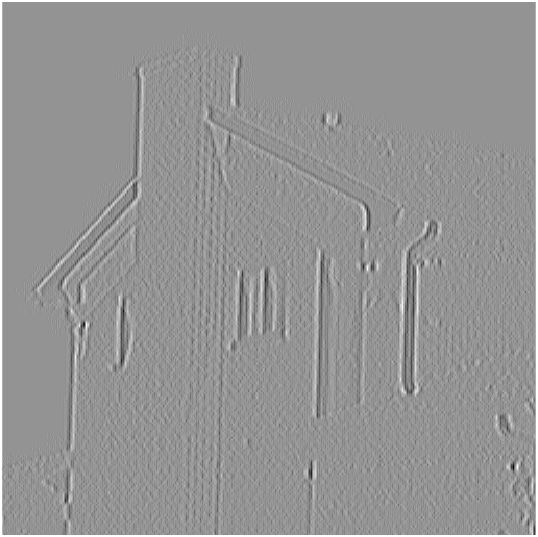
\includegraphics[width=0.4\textwidth]{images/p3c/laplacian_res_y.png}
			\label{fig:laplacian_res_y}
		}
		\caption{Those images are processed to map their original value interval to $[0, 255]$ for visualization purposes.}
	\end{figure}
	\item [(d)] Results after applying LoG filter and unsharpen mask are shown in~\ref{fig:LoG_res_1}~\ref{fig:LoG_res_0.5}~\ref{fig:LoG_res_0.25} and~\ref{fig:unsharpen_res} respectively.
	\begin{figure}
		\centering
		\subfigure[Result after applying LoG filter with $\sigma=1$]{
			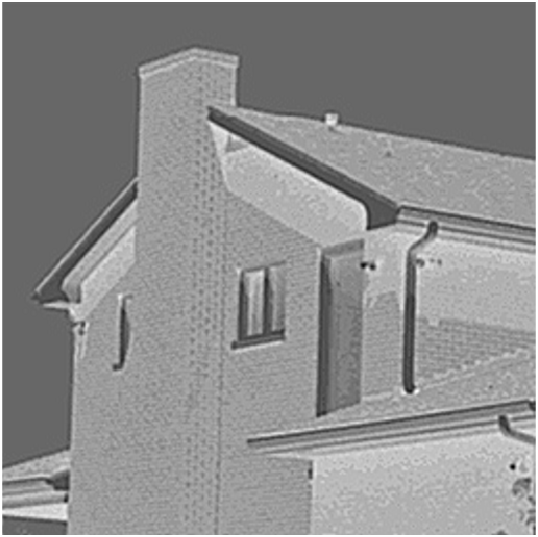
\includegraphics[width=0.4\textwidth]{images/p3d/LoG_res.png}
			\label{fig:LoG_res_1}
		}
		\subfigure[Result after applying LoG filter with $\sigma=0.5$]{
			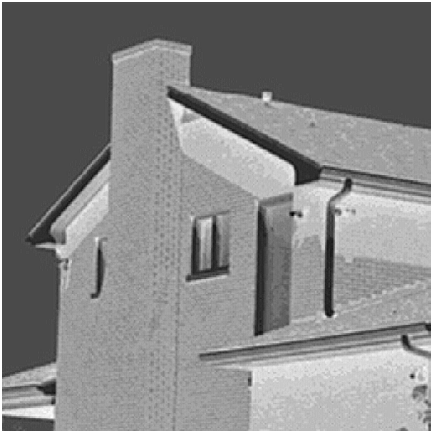
\includegraphics[width=0.4\textwidth]{images/p3d/LoG_res_0.5.png}
			\label{fig:LoG_res_0.5}
		}
		\subfigure[Result after applying LoG filter with $\sigma=0.25$]{
			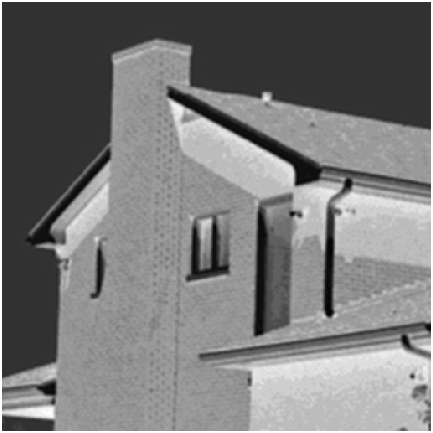
\includegraphics[width=0.4\textwidth]{images/p3d/LoG_res_0.25.png}
			\label{fig:LoG_res_0.25}
		}
		\subfigure[Result after applying unsharpen mask]{
			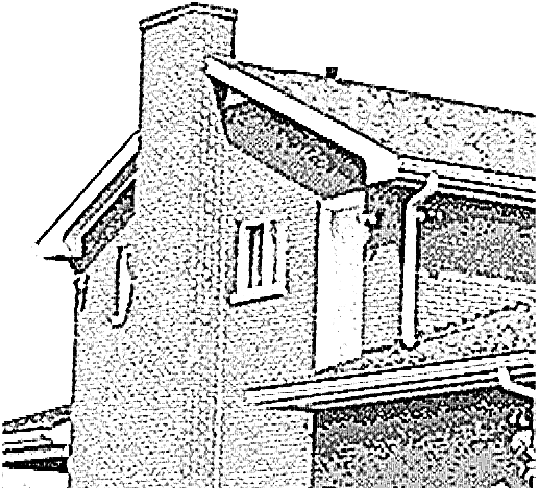
\includegraphics[width=0.4\textwidth]{images/p3d/unsharpen_res.png}
			\label{fig:unsharpen_res}
		}
		\caption{The Result of LoG filter is processed to fit intensity interval $[0, 255]$ for visualization purposes. The unsharpen mask uses Gaussian kernel to get the smooth image and sets $k=100$}
	\end{figure}
\end{itemize}

\end{document}
